\documentclass[11pt]{article}

% -------------------------------------------------
% Idioma y codificación
% -------------------------------------------------
\usepackage[utf8]{inputenc}
\usepackage[T1]{fontenc}
\usepackage[spanish,mexico]{babel}

% -------------------------------------------------
% Tipografía y composición
% -------------------------------------------------
\usepackage{lmodern}
\usepackage{microtype}
\usepackage{setspace}
\usepackage{xurl}

% -------------------------------------------------
% Márgenes
% -------------------------------------------------
\usepackage[
    top=2.5cm,
    bottom=2.5cm,
    left=2.7cm,
    right=2.7cm
]{geometry}

% -------------------------------------------------
% Tablas, figuras y listas
% -------------------------------------------------
\usepackage{booktabs}
\usepackage{tabularx}
\usepackage{longtable}
\usepackage{array}
\usepackage{graphicx}
\usepackage{caption}
\usepackage{enumitem}
\usepackage{float}

% -------------------------------------------------
% Matemáticas
% -------------------------------------------------
\usepackage{amsmath}
\usepackage{amssymb}

% -------------------------------------------------
% Referencias
% -------------------------------------------------
\usepackage{csquotes}
\usepackage[
    backend=biber,
    style=apa,
    sorting=nyt
]{biblatex}

\addbibresource{referencias.bib}

% -------------------------------------------------
% Hipervínculos
% -------------------------------------------------
\usepackage[
    hidelinks
]{hyperref}

% -------------------------------------------------
% Formato general
% -------------------------------------------------
\setstretch{1.15}

\setlength{\parindent}{0pt}
\setlength{\parskip}{0.6em}

\setlist[itemize]{
    leftmargin=*,
    topsep=0.3em,
    itemsep=0.2em
}

\setlist[enumerate]{
    leftmargin=*,
    topsep=0.3em,
    itemsep=0.2em
}

\usepackage{placeins}
% -------------------------------------------------
% Documento
% -------------------------------------------------
\begin{document}

% -------------------------------------------------
% Portada
% -------------------------------------------------
\begin{titlepage}
    \centering

    \vspace*{2.0cm}

    {\large\bfseries
    Avance 3
    \par}

    \vspace{0.6cm}

    {\LARGE\bfseries
    \parbox{0.88\textwidth}{
        \centering
        Baseline para la reconstrucción de matrices de tiempos de viaje
    }
    \par}

    \vspace{1.2cm}

    {\large
    \parbox{0.88\textwidth}{
        \centering
        Planeación inteligente de rutas ante interrupciones mediante técnicas de optimización e inteligencia artificial
    }
    \par}

    \vspace{1.5cm}

    {\large\bfseries
    Equipo 42 -- Route Intelligence
    \par}

    \vspace{0.35cm}

    {\normalsize
    Maestría en Inteligencia Artificial Aplicada
    \par}

    \vspace{1.5cm}

    {\normalsize
    Luis Ángel Herrera Flores\\[0.25cm]
    Francisco Natanael Ortiz Martínez\\[0.25cm]
    Edgar Iván Rosas Gómez
    \par}

    \vspace{1.2cm}

    {\normalsize
    Asesor / Sponsor: Dr. Gerardo Jesús Camacho González
    \par}

    \vfill

    {\normalsize
    Octubre de 2026
    \par}

\end{titlepage}

% -------------------------------------------------
% Índice
% -------------------------------------------------
\tableofcontents
\newpage

\section{Introducción y objetivo del avance}

El Proyecto Integrador aborda la planeación y replaneación de rutas ante interrupciones en problemas de ruteo de vehículos con ventanas de tiempo. El problema de interés no se limita a obtener una planeación inicial eficiente, sino a determinar cómo adaptar una operación que ya se encuentra en ejecución cuando cambian las condiciones bajo las cuales fue construida. Como principal modelo de referencia se considera el enfoque desarrollado por Berth y Trigos, en el que una solución inicialmente factible puede requerir ser recalculada cuando modificaciones en los tiempos de viaje comprometen el cumplimiento de las ventanas de tiempo \parencite{berth_thesis_2025,berth_trigos_2025}.

En este esquema, la matriz de tiempos de viaje $T=[t_{ij}]$ constituye una entrada del problema de optimización, donde cada elemento $t_{ij}$ representa el tiempo asociado con la transición del nodo $i$ al nodo $j$. A partir de esta matriz se construye la planeación previa a la operación; durante la ejecución, las modificaciones en las condiciones de movilidad pueden representarse mediante una matriz actualizada $T'$. Esta información se utiliza para monitorear la factibilidad de las rutas y, cuando una desviación conduce a una futura violación de las ventanas de tiempo, identificar un tiempo de interrupción $t_D$. A partir del estado alcanzado en ese instante se construye una instancia residual que preserva las decisiones ya ejecutadas y permite recalcular la parte pendiente de la operación \parencite{berth_thesis_2025,berth_trigos_2025}.

Los avances anteriores permitieron identificar la actualización de esta información temporal como un punto de intervención particularmente relevante para el componente de inteligencia artificial. Esta delimitación responde también a una necesidad práctica planteada durante las sesiones de trabajo con el asesor del Proyecto, Dr. Gerardo Jesús Camacho González, y con los doctores Federico Trigos Salazar y Mario Alberto Doria Serrano, investigadores con experiencia en optimización y problemas de ruteo: aunque el modelo de optimización puede operar a partir de una matriz completa de tiempos entre los puntos de la instancia, obtener dicha matriz con información suficientemente representativa de las condiciones de movilidad puede convertirse en un cuello de botella, especialmente cuando cambian las condiciones de movilidad y el tiempo disponible para reaccionar es reducido. En este contexto se distinguen dos momentos relacionados pero diferentes: la planeación previa al turno, en la que existe un horizonte mayor para anticipar las condiciones esperadas, y la recuperación durante la ejecución, en la que interesa actualizar con rapidez los tiempos correspondientes a los servicios aún pendientes.

El Avance 2 delimitó el segundo escenario como el principal objeto del diseño experimental. La propuesta consiste en aprender previamente la estructura recurrente de las condiciones de movilidad a partir de información histórica y, durante la operación, utilizar un número reducido de observaciones actuales para estimar los tiempos que no pueden consultarse directamente. De esta forma, el componente de estimación no sustituye el mecanismo de optimización y recuperación, sino que busca proporcionar de manera oportuna una representación más informativa de los tiempos de viaje que posteriormente puede ser utilizada por dicho mecanismo.

El presente avance establece el primer nivel de referencia para evaluar este componente. Se define el escenario $K=0$, en el que el método de estimación no dispone de observaciones actuales de tiempos de recorrido y debe reconstruir los tiempos origen--destino exclusivamente a partir de la información histórica disponible. Este escenario no constituye el baseline global del problema de replaneación, sino la referencia del componente de estimación frente a la cual se evaluará posteriormente el valor adicional aportado por un número reducido de observaciones actuales, $K>0$.

Para construir esta referencia se utiliza PEMS-BAY como entorno experimental, un conjunto de datos de tráfico derivado del Performance Measurement System (PeMS) del California Department of Transportation que contiene series históricas de velocidad registradas por sensores de autopistas del Área de la Bahía de San Francisco. A partir de estas observaciones se obtiene una representación dinámica de una red dirigida y, para cada instante disponible, una matriz de tiempos de desplazamiento entre 13 macronodos. Sobre esta secuencia temporal se analizan los patrones relevantes para la estimación, se comparan diferentes referencias históricas y se selecciona una especificación mediante un conjunto de validación independiente. Finalmente, el baseline elegido se evalúa sobre un periodo de prueba no utilizado durante la selección.

El objetivo de este avance es, por tanto, establecer un nivel de desempeño simple, interpretable y reproducible para la estimación de la matriz de tiempos de viaje cuando no se dispone de información actual. Además de proporcionar una referencia cuantitativa para las siguientes etapas, este análisis permite caracterizar qué parte de la variación de los tiempos puede explicarse mediante patrones históricos y establecer el punto de comparación necesario para estudiar posteriormente cuánto valor aportan unas pocas observaciones actuales al proceso de reconstrucción y, en una etapa posterior, a la recuperación de las rutas.

\section{Punto de integración y entorno experimental}
\subsection{Papel de la matriz de tiempos de viaje en la planeación y recuperación}

En el modelo de referencia, la planeación de las rutas requiere conocer los tiempos asociados con las transiciones entre los nodos de la instancia. Berth representa esta información mediante una matriz

\[
T=[t_{ij}],
\]

donde cada elemento $t_{ij}$ corresponde al tiempo asociado con la transición del nodo $i$ al nodo $j$. Bajo la convención utilizada en su formulación, el tiempo de servicio $s_j$ se encuentra incorporado en $t_{ij}$ \parencite{berth_thesis_2025}. Para distinguir la parte asociada específicamente con la movilidad, en este Proyecto se utiliza $\tau_{ij}$ para denotar el tiempo de desplazamiento entre ambos nodos, de modo que conceptualmente puede escribirse

\[
t_{ij}=\tau_{ij}+s_j.
\]

Esta separación resulta relevante porque los tiempos de servicio corresponden a características de la operación logística, mientras que $\tau_{ij}$ depende de las condiciones de movilidad y puede variar durante la ejecución. El componente desarrollado en esta etapa del Proyecto se concentra en estimar estos tiempos de desplazamiento; posteriormente, dicha información puede integrarse con los demás parámetros requeridos por el modelo de ruteo.

Durante la ejecución, el modelo de Berth representa los cambios en las condiciones de viaje mediante desviaciones $\Delta t_{ij}$ sobre los tiempos inicialmente considerados. Una vez conocidos estos cambios, se obtiene una matriz modificada $T'$, que es utilizada por el procedimiento de monitoreo de factibilidad. En los experimentos de la tesis, dichas desviaciones no son estimadas a partir de observaciones de tráfico, sino generadas de manera exógena mediante una simulación estocástica de eventos de congestión \parencite{berth_thesis_2025}. Por tanto, el modelo establece cómo utilizar una matriz de tiempos modificada, pero no aborda el problema de inferir oportunamente sus valores cuando sólo se dispone de información parcial sobre las condiciones actuales de movilidad.

A partir de $T'$, el procedimiento de monitoreo examina la parte pendiente de las rutas y evalúa cómo se propagan los retrasos. Si las holguras disponibles permiten absorber las desviaciones, la planeación puede mantenerse. Si, por el contrario, la propagación conduce a una futura violación de una ventana de tiempo, el procedimiento identifica un tiempo de interrupción $t_D$ \parencite{berth_thesis_2025,berth_trigos_2025}.

Una vez identificado $t_D$, el mecanismo de recuperación considera el estado alcanzado por la operación en dicho instante. Las decisiones ya ejecutadas se preservan, la instancia original se ajusta para representar únicamente la parte aún pendiente y se construye una instancia residual sobre la cual puede realizarse la reoptimización. Dependiendo de la severidad de las condiciones modificadas, la recuperación puede mantener la formulación original del VRPTW o requerir las medidas adicionales contempladas por el DVRPTW \parencite{berth_thesis_2025,berth_trigos_2025}.

El presente Proyecto interviene antes de estas etapas de monitoreo y recuperación. En lugar de suponer disponible la totalidad de los tiempos actuales, se busca estimar la información de movilidad requerida a partir de la estructura histórica aprendida y, en etapas posteriores, de un número reducido de observaciones actuales. El objetivo no es sustituir el procedimiento que determina si una desviación constituye una interrupción ni el mecanismo posterior de recuperación, sino proporcionar oportunamente los tiempos que dichos procedimientos necesitan. Esta necesidad coincide con el problema práctico identificado durante las sesiones de trabajo del Proyecto: en una operación real, obtener individualmente los tiempos actuales para todos los pares origen--destino puede consumir una parte importante del tiempo disponible para reaccionar.

Para mantener separada esta etapa de la formulación logística de Berth, se denotará mediante

\[
T^{\tau}(t)=\left[\tau_{ij}(t)\right]
\]

la matriz de tiempos de desplazamiento correspondiente al estado de movilidad de la red en el instante $t$. Esta matriz constituye el objeto de estimación en el entorno experimental desarrollado para este avance. Su estimación proporciona la información temporal que, en una integración posterior, puede utilizarse para actualizar los valores empleados por el modelo de ruteo antes del monitoreo de factibilidad y de una eventual recuperación.

\subsection{Construcción de la red experimental y de las matrices de tiempos}

PEMS-BAY proporciona observaciones históricas de velocidad registradas por sensores instalados en autopistas del área de la Bahía de San Francisco, pero su estructura no corresponde directamente a la de una instancia de ruteo. En particular, los datos originales describen velocidades en puntos instrumentados de la red y no tiempos de desplazamiento entre los nodos que posteriormente utilizaría un modelo de optimización. La versión empleada en este Proyecto contiene información de 325 sensores y 52\,116 instantes comprendidos entre el 1 de enero y el 30 de junio de 2017, con una frecuencia nominal de cinco minutos \parencite{caltrans_pems,li2018dcrnn}. Por ello, fue necesario construir a partir de estas observaciones un entorno experimental que permitiera representar recorridos dirigidos y obtener matrices origen--destino de tiempos de desplazamiento.

Además de las series temporales de velocidad, se utilizaron dos archivos de metadatos procedentes del repositorio público \textit{Augmented PEMS-BAY}: \path{sensor_metadata.csv} y \path{freeway_sensor_sequence.csv} \parencite{augmented_pems_bay}. El primero proporciona, para cada sensor, información como la autopista y el sentido de circulación asociados, el \textit{postmile}, que indica su posición longitudinal a lo largo de la autopista mediante una referencia expresada en millas, las coordenadas geográficas, la longitud del segmento representado y el número de carriles. El segundo proporciona el orden de los sensores dentro de cada corredor dirigido.

Antes de utilizar las velocidades en la construcción de la red se revisó la calidad y continuidad temporal del conjunto. No se identificaron valores ausentes en la matriz original. Al comparar las marcas temporales con una rejilla regular de cinco minutos se observaron 12 intervalos aparentemente ausentes, todos ellos entre las 02:00 y las 02:55 del 12 de marzo de 2017. Esta discontinuidad coincide con el inicio del horario de verano en California, cuando la hora local avanza directamente de las 02:00 a las 03:00, por lo que no se interpretó como pérdida de observaciones.

También se identificaron 521 valores de velocidad iguales a cero, equivalentes aproximadamente al 0.0031\,\% de las observaciones sensor--tiempo. Estos valores se concentraron exclusivamente en cuatro instantes, en los que aparecieron simultáneamente en un número elevado de sensores, por lo que se consideraron observaciones anómalas asociadas con el proceso de adquisición o preprocesamiento. El conjunto original se conservó sin modificaciones y, en la copia de trabajo utilizada en los experimentos, estos valores se trataron como datos ausentes y se estimaron mediante interpolación temporal entre las observaciones válidas inmediatamente adyacentes de cada sensor.

A partir de los metadatos se organizaron los 325 sensores en 16 corredores dirigidos, correspondientes a los dos sentidos de circulación de ocho autopistas. La variable que define su orden dentro de cada corredor no presentó duplicados ni discontinuidades y las secuencias resultantes mostraron una disposición espacial consistente con las autopistas representadas. Los sensores consecutivos dentro de cada corredor se conectaron mediante aristas dirigidas que conservan explícitamente el sentido de circulación.

Los metadatos de PEMS-BAY no especifican por sí solos todas las conexiones posibles entre corredores. Por esta razón, OpenStreetMap se utilizó como fuente auxiliar para inspeccionar la infraestructura vial alrededor de los corredores e identificar zonas plausibles de intercambio \parencite{openstreetmap}. La presencia de una intersección o enlace en OpenStreetMap no implicó su incorporación automática a la red experimental. Para cada zona candidata se examinó conjuntamente la proximidad de los sensores disponibles, su posición dentro del corredor y la continuidad vial observada alrededor del intercambio. La decisión de anclaje no se basó, por tanto, en un umbral fijo de distancia: algunos corredores relativamente alejados pudieron conservarse cuando la separación correspondía a un tramo terminal no instrumentado, mientras que otros se descartaron cuando la cobertura disponible no permitía representar razonablemente una conexión local con la zona de intercambio.

Las zonas seleccionadas se representaron mediante 13 macronodos. Un macronodo no corresponde a una rampa específica ni a un punto físico exacto de la infraestructura, sino a una abstracción funcional que permite conectar los corredores dirigidos asociados con una misma zona de intercambio. Para cada combinación entre macronodo y corredor se identificaron los sensores utilizados para ingresar a la zona y para abandonarla.

Dentro de esta abstracción, una trayectoria que llega al macronodo por cualquiera de sus aristas de entrada puede continuar por cualquiera de sus aristas de salida. No se representan de manera individual las restricciones de movimiento dentro del intercambio ni se asigna un tiempo adicional a la transición interna. Esta simplificación permite construir una representación funcional y conectada de las zonas de intercambio, pero puede admitir movimientos que en la infraestructura vial real estarían sujetos a restricciones específicas. En consecuencia, los macronodos deben interpretarse como elementos del entorno experimental y no como una reconstrucción detallada de cada maniobra vial.

La red resultante es dirigida: los sensores correspondientes a sentidos opuestos de una misma autopista pertenecen a corredores diferentes y sus conexiones conservan explícitamente esta orientación. Esta característica es necesaria porque tanto los recorridos disponibles como las condiciones de movilidad pueden diferir según el sentido de circulación.

Para facilitar la interpretación espacial de la estructura construida se utiliza la representación mostrada en la Figura~\ref{fig:red_experimental}. Debido a que los sensores correspondientes a sentidos opuestos de una misma autopista se encuentran geográficamente muy próximos, al utilizar directamente sus coordenadas ambas secuencias tienden a superponerse. Únicamente con fines de visualización, los sensores se desplazan ligeramente en direcciones opuestas de acuerdo con el sentido de circulación. Esta separación gráfica no modifica las coordenadas utilizadas en los cálculos, la conectividad del grafo, las longitudes de las aristas ni los tiempos de desplazamiento.

\begin{figure}[H]
    \centering
    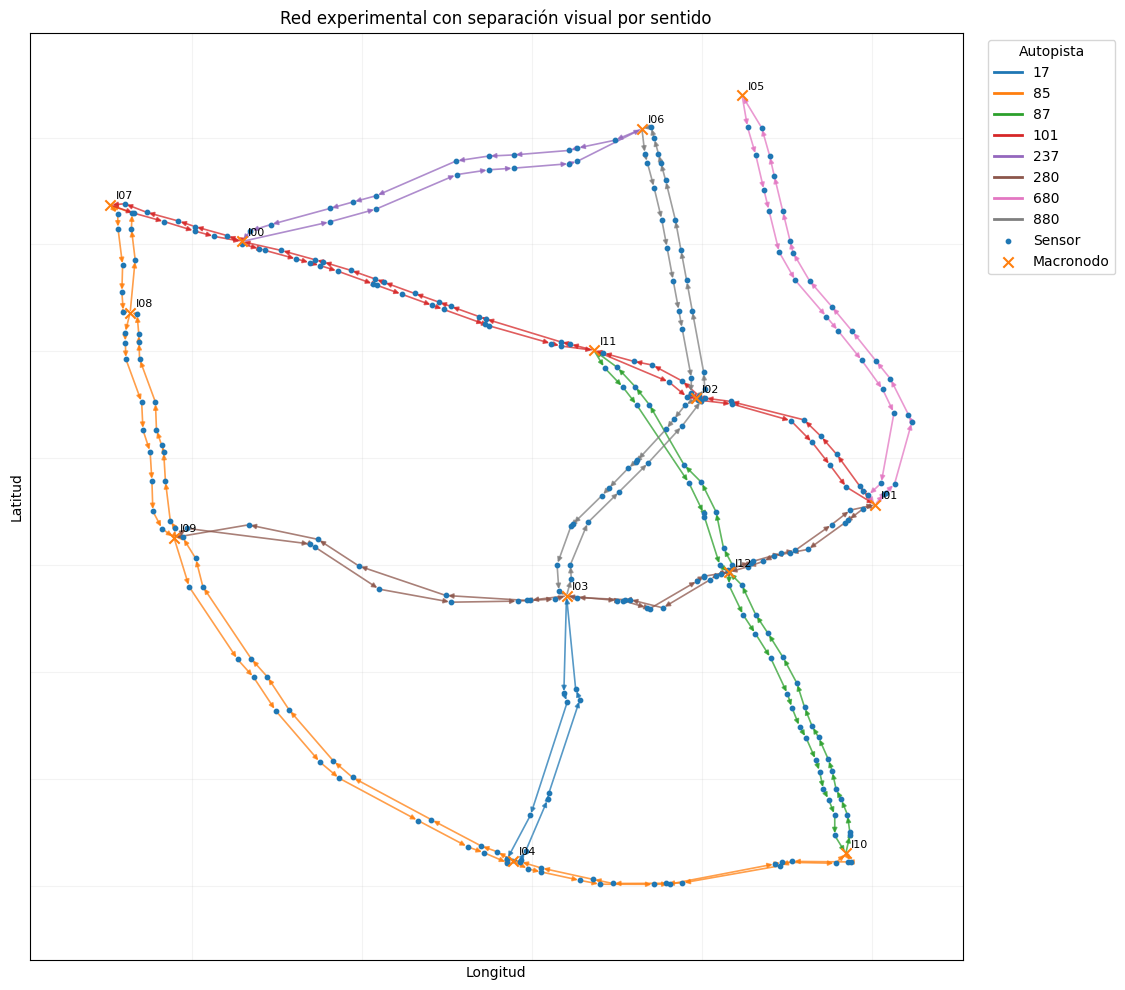
\includegraphics[width=0.92\textwidth]{figuras/red_experimental_dirigida.png}
    \caption{Representación de la red experimental dirigida construida a partir de PEMS-BAY. Los macronodos representan zonas funcionales de intercambio entre corredores. Para distinguir visualmente los sentidos opuestos de una misma autopista se aplica una pequeña separación artificial entre sus sensores; este ajuste afecta únicamente la representación gráfica y no la red utilizada en los cálculos.}
    \label{fig:red_experimental}
\end{figure}

Una vez incorporadas las conexiones entre corredores y macronodos, se identificó el principal componente fuertemente conexo del grafo. Esta delimitación garantiza que, dentro de la red utilizada en los experimentos, exista al menos una trayectoria dirigida entre cualquier par de nodos del núcleo. El componente resultante contiene 322 nodos: 309 sensores PEMS-BAY y los 13 macronodos, conectados mediante 345 aristas dirigidas. Los 16 sensores que quedaron fuera de esta componente permanecen disponibles en el conjunto de datos original, pero no intervienen en la construcción de las trayectorias ni de las matrices de tiempos utilizadas posteriormente.

Para transformar la estructura espacial en tiempos de recorrido se asignó una longitud a cada una de las 345 aristas del núcleo. En las aristas entre sensores consecutivos de un mismo corredor, la longitud se obtuvo a partir de la diferencia absoluta de sus valores de \textit{postmile}, convertida de millas a kilómetros. Si $p_u$ y $p_v$ representan los valores de \textit{postmile} de dos sensores consecutivos,

\[
d_{uv}
=
|p_v-p_u|\,1.609344.
\]

Cuando un macronodo se inserta entre dos sensores consecutivos, se conserva la longitud total del segmento original y se divide entre las dos nuevas conexiones de acuerdo con la proximidad geográfica del macronodo a ambos extremos. Para los anclajes situados antes del inicio o después del final de la cobertura instrumentada, donde no existe un segmento original que pueda dividirse, la longitud se aproxima mediante la distancia geodésica entre el sensor terminal y el macronodo. En el núcleo final, 273 aristas conservan directamente una distancia derivada de \textit{postmile}, 49 corresponden a segmentos divididos por la inserción de macronodos y 23 a conexiones terminales aproximadas geodésicamente.

A cada arista se le asignó también una serie temporal de velocidad. Cuando una arista $(u,v)$ conecta dos sensores PEMS-BAY, la velocidad se aproxima mediante el promedio de las velocidades observadas en ambos extremos,

\[
v_{uv}(t)
=
\frac{v_u(t)+v_v(t)}{2}.
\]

Cuando una conexión involucra un macronodo, solamente el extremo correspondiente al sensor dispone de una observación de velocidad. En estos casos se utiliza la velocidad del sensor asociado, ya que el macronodo representa una zona funcional de intercambio y no un punto adicional de medición.

Las velocidades originales de PEMS-BAY se encuentran expresadas en millas por hora. Si $d_{uv}$ denota la longitud de la arista $(u,v)$ en kilómetros, su tiempo de desplazamiento se calcula como

\[
\tau_{uv}(t)
=
60
\frac{d_{uv}}
     {1.609344\,v_{uv}(t)},
\]

donde $\tau_{uv}(t)$ queda expresado en minutos. Este procedimiento produce una serie temporal de tiempos de desplazamiento para cada una de las 345 aristas del núcleo y conserva la resolución temporal nominal de cinco minutos.

A partir de estos tiempos por arista puede construirse, para cualquier instante $t$ y para cualquier conjunto de nodos de interés, una matriz dirigida de tiempos de desplazamiento. En el entorno experimental, la matriz calculada utilizando la totalidad de las observaciones disponibles en un instante se utiliza como referencia y se denota mediante

\[
T^\tau_{\mathrm{ref}}(t)
=
\left[
T^\tau_{\mathrm{ref},ij}(t)
\right].
\]

Para cada par ordenado de nodos $(i,j)$, el elemento $T^\tau_{\mathrm{ref},ij}(t)$ corresponde al tiempo mínimo de desplazamiento entre ambos nodos,

\[
T^\tau_{\mathrm{ref},ij}(t)
=
\min_{p\in\mathcal{P}_{ij}}
\sum_{(u,v)\in p}
\tau_{uv}(t),
\]

donde $\mathcal{P}_{ij}$ representa el conjunto de caminos dirigidos disponibles entre $i$ y $j$. El cálculo se realiza mediante el algoritmo de Dijkstra \parencite{dijkstra1959note}, utilizando como peso de cada arista su tiempo de desplazamiento $\tau_{uv}(t)$. Dado que los pesos son no negativos, el algoritmo permite obtener los tiempos mínimos desde cada origen hacia los demás nodos alcanzables.

En esta etapa se adopta una representación \textit{snapshot}. Para construir $T^\tau_{\mathrm{ref}}(t)$, los tiempos de todas las aristas se fijan en los valores correspondientes al instante $t$ durante todo el cálculo del camino mínimo. Por tanto, cada matriz representa el estado de movilidad de la red en ese instante y no incorpora todavía la posible evolución de las condiciones de tráfico mientras un vehículo se encuentra recorriendo una trayectoria.

Para mantener una distinción explícita respecto de la matriz $T$ del modelo de Berth, cuyos elementos incorporan además el tiempo de servicio, en este documento se utiliza el superíndice $\tau$ para identificar matrices compuestas exclusivamente por tiempos de desplazamiento. En los cuadernos computacionales que acompañan este avance, la construcción anterior aparece inicialmente como $T(t)$ y, cuando se utiliza como referencia experimental completamente observada, como $T_{\mathrm{ref}}(t)$. Por tanto, $T_{\mathrm{ref}}(t)$ en la implementación corresponde a $T^\tau_{\mathrm{ref}}(t)$ en la notación utilizada en este documento; la diferencia es exclusivamente notacional.

Una vez construida la red y definido el procedimiento para obtener tiempos de recorrido sobre ella, es necesario determinar qué nodos desempeñarán el papel de orígenes y destinos de la matriz experimental. Para este avance se utilizan los 13 macronodos, con el propósito de disponer de un conjunto de referencia reducido y funcionalmente interpretable sin hacer coincidir el tamaño de la matriz con el número de puntos instrumentados. Los sensores PEMS-BAY proporcionan las observaciones de tráfico y forman parte de la estructura interna sobre la que se calculan los recorridos, mientras que los macronodos actúan como puntos de referencia para los tiempos origen--destino que serán objeto de estimación.

Esta elección corresponde exclusivamente a la configuración experimental desarrollada en este avance. Los macronodos no se interpretan como clientes, depósitos u otras ubicaciones logísticas reales y su utilización no restringe la formulación general del problema. En etapas posteriores, el conjunto de nodos origen--destino podría ampliarse con sensores seleccionados, combinar sensores y macronodos o incluso definirse únicamente a partir de sensores, dependiendo del objetivo del experimento y de la correspondencia que se busque establecer con una aplicación logística concreta.

En consecuencia, cada instante produce una matriz dirigida de $13\times13$, con 13 elementos diagonales iguales a cero y 156 pares origen--destino no diagonales. Debido a que la red conserva explícitamente el sentido de circulación, no se impone simetría entre estos tiempos y, en general,

\[
T^\tau_{\mathrm{ref},ij}(t)
\neq
T^\tau_{\mathrm{ref},ji}(t).
\]

Esta característica permite conservar las diferencias de movilidad entre sentidos y constituye la representación de referencia sobre la que se desarrollan los análisis y experimentos de estimación descritos en las secciones siguientes.

\subsection{Representación temporal y variable objetivo}

La construcción descrita en la sección anterior permite obtener una matriz de referencia $T^{\tau}_{\mathrm{ref}}(t)$ para cualquier instante disponible en PEMS-BAY. Sin embargo, el objetivo experimental no consiste en analizar una única condición de la red, sino en aprovechar la repetición temporal de estas matrices para aprender patrones históricos que permitan estimar los tiempos de desplazamiento cuando no se dispone de información actual completa.

Para ello, el procedimiento se aplica a cada uno de los 52\,116 instantes disponibles entre el 1 de enero y el 30 de junio de 2017. En cada instante $t_n$ se utilizan los tiempos correspondientes a las 345 aristas del núcleo de enrutamiento y se calculan los caminos de tiempo mínimo entre los 13 macronodos. Como resultado se obtiene una secuencia

\[
T^{\tau}_{\mathrm{ref}}(t_1),
T^{\tau}_{\mathrm{ref}}(t_2),
\ldots,
T^{\tau}_{\mathrm{ref}}(t_N),
\]

con $N=52\,116$. Esta secuencia puede representarse mediante un tensor temporal

\[
\mathcal{T}^{\tau}_{\mathrm{ref}}
\in
\mathbb{R}^{N\times13\times13},
\]

donde la primera dimensión corresponde al tiempo y las dos restantes identifican el origen y el destino dentro del conjunto de macronodos. En el experimento desarrollado,

\[
\mathcal{T}^{\tau}_{\mathrm{ref}}
\in
\mathbb{R}^{52\,116\times13\times13}.
\]

Las entradas diagonales de cada matriz son iguales a cero, puesto que no existe tiempo de desplazamiento de un nodo hacia sí mismo. En consecuencia, cada matriz contiene 156 pares origen--destino dirigidos con información relevante,

\[
13(13-1)=156.
\]

Cada uno de estos pares se considera una variable de tiempo de desplazamiento distinta. Esta distinción es importante porque la red es dirigida y, por tanto, los pares $(i,j)$ y $(j,i)$ representan variables diferentes que pueden seguir patrones temporales distintos.

Aunque la representación tensorial conserva de manera natural la estructura de las matrices origen--destino, para la construcción y evaluación del baseline resulta conveniente utilizar también una representación tabular equivalente. Para cada instante se extraen únicamente las 156 entradas no diagonales de $T^{\tau}_{\mathrm{ref}}(t)$, de modo que cada fila del conjunto de datos corresponde a un instante y cada columna a un par origen--destino dirigido. El conjunto resultante puede representarse de manera esquemática como

\[
Y_{\mathrm{ref}}
=
\begin{bmatrix}
T^{\tau}_{\mathrm{ref},1}(t_1) &
T^{\tau}_{\mathrm{ref},2}(t_1) &
\cdots &
T^{\tau}_{\mathrm{ref},156}(t_1)
\\
T^{\tau}_{\mathrm{ref},1}(t_2) &
T^{\tau}_{\mathrm{ref},2}(t_2) &
\cdots &
T^{\tau}_{\mathrm{ref},156}(t_2)
\\
\vdots & \vdots & \ddots & \vdots \\
T^{\tau}_{\mathrm{ref},1}(t_N) &
T^{\tau}_{\mathrm{ref},2}(t_N) &
\cdots &
T^{\tau}_{\mathrm{ref},156}(t_N)
\end{bmatrix},
\]

donde cada columna conserva la correspondencia con un par ordenado $(i,j)$ específico. Esta transformación no modifica la información de las matrices originales; únicamente reorganiza las entradas relevantes en un formato conveniente para construir referencias históricas y calcular métricas de error.

La variable objetivo del componente de estimación es, por tanto, el tiempo de desplazamiento correspondiente a cada uno de estos 156 pares origen--destino en un instante determinado. En el escenario $K=0$, definido en la sección introductoria, ninguna entrada actual de $T^{\tau}_{\mathrm{ref}}(t)$ se proporciona al método de estimación. Para un instante $t$, el baseline debe producir una matriz estimada

\[
\widehat{T}^{\tau,(0)}(t),
\]

utilizando exclusivamente la información histórica disponible antes del periodo que se desea estimar.

La matriz completa $T^{\tau}_{\mathrm{ref}}(t)$ se conserva únicamente como referencia experimental para evaluar estas estimaciones. En una aplicación real no se supondría disponible durante la inferencia, ya que conocer todas sus entradas eliminaría precisamente el problema de estimación planteado. La disponibilidad completa de las observaciones en PEMS-BAY permite, en este entorno controlado, ocultar deliberadamente la información actual y posteriormente comparar las estimaciones con los valores que efectivamente se obtienen al utilizar todas las observaciones de tráfico.

Esta separación entre información disponible para estimar e información utilizada únicamente para evaluar será también la base del escenario posterior $K>0$. En ese caso se incorporará un conjunto reducido de $K$ observaciones actuales de tiempos de recorrido correspondientes a pares seleccionados de la red experimental. Los pares observados podrán coincidir total o parcialmente con los pares origen--destino de la matriz objetivo, o corresponder a otros puntos de la red, dependiendo del método de reconstrucción y de la estrategia de selección de observaciones que se adopten posteriormente. A partir de estas observaciones y de la estructura histórica aprendida previamente, se buscará actualizar la estimación histórica $\widehat{T}^{\tau,(0)}(t)$ y obtener una reconstrucción de los tiempos origen--destino requeridos. La matriz completa $T^\tau_{\mathrm{ref}}(t)$ permanecerá disponible únicamente como referencia experimental para evaluar la calidad de la reconstrucción.

El desempeño obtenido se comparará con el nivel de referencia establecido por $K=0$, con el fin de cuantificar cuánto valor adicional aporta disponer de una cantidad limitada de información actual.

\section{Evidencia exploratoria relevante para el baseline}

\subsection{Estructura temporal}

Antes de construir el baseline $K=0$ resulta necesario determinar si los datos presentan regularidades temporales que puedan ser aprovechadas para estimar los tiempos de desplazamiento a partir de información histórica. Si las condiciones de movilidad fueran independientes de la hora o del tipo de día, utilizar estas variables para definir referencias históricas no aportaría información adicional respecto de una estimación global.

Para examinar esta estructura se utilizó la información de las 345 aristas dirigidas de la red experimental. En cada instante se calculó una velocidad representativa de la red mediante la mediana de las velocidades de dichas aristas. El uso de la mediana permite resumir el estado general de la red reduciendo la influencia de valores extremos asociados con segmentos particulares. Posteriormente, las observaciones se agruparon de acuerdo con la hora del día y se distinguieron dos tipos de día: laborables, de lunes a viernes, y fines de semana, correspondientes a sábado y domingo.

La Figura~\ref{fig:perfil_horario} muestra el perfil horario obtenido para ambas categorías. Cada punto representa la mediana de la velocidad representativa de la red observada en una determinada hora a lo largo del periodo analizado.

\begin{figure}[H]
    \centering
    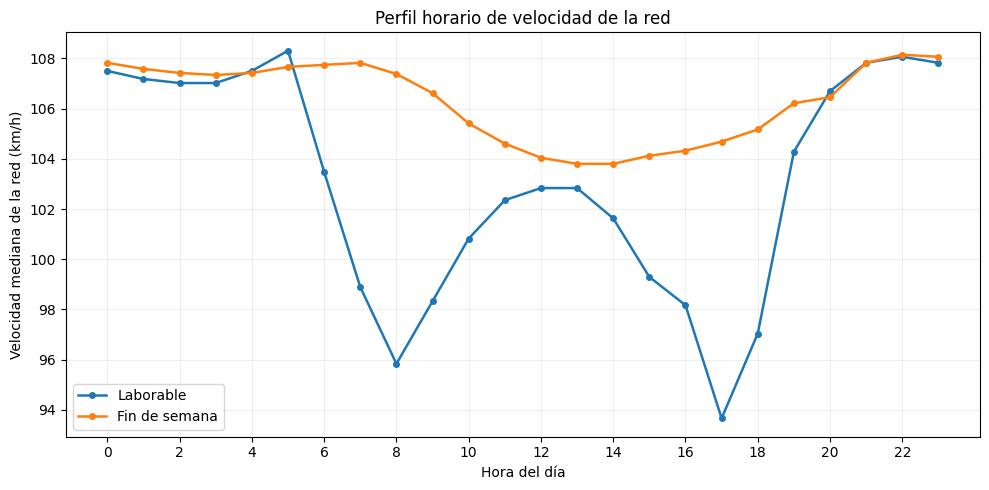
\includegraphics[width=0.88\textwidth]{figuras/perfil_horario_laborable_fin_semana.png}
    \caption{Perfil horario de la velocidad representativa de la red para días laborables y fines de semana. La velocidad representativa de cada instante corresponde a la mediana de las velocidades de las 345 aristas dirigidas.}
    \label{fig:perfil_horario}
\end{figure}

El comportamiento observado evidencia una estructura temporal diferenciada. Durante los días laborables aparecen reducciones de velocidad asociadas con los periodos de mayor congestión, particularmente alrededor de las horas pico de la mañana y de la tarde, mientras que durante los fines de semana el perfil es comparativamente más estable. Por tanto, una misma ubicación temporal dentro del día no necesariamente representa condiciones equivalentes cuando cambia el tipo de día.

Esta evidencia sugiere que una referencia histórica que ignore completamente la posición temporal de una observación puede mezclar estados de movilidad sistemáticamente distintos. En consecuencia, la hora del día y la posición de la observación dentro de la semana constituyen variables temporalmente informativas que conviene evaluar en la construcción del baseline. Esta conclusión no implica todavía que una determinada combinación de variables o granularidad temporal sea óptima; únicamente justifica evaluar progresivamente referencias históricas que incorporen esta información.

La comparación posterior de especificaciones permitirá cuantificar este efecto. En particular, se partirá de una referencia histórica sin diferenciación temporal y se evaluará cuánto mejora la estimación al incorporar primero la hora del día y posteriormente el día de la semana. De esta forma, la relevancia de estas variables no se establecerá únicamente a partir de la inspección gráfica, sino también mediante su efecto sobre el error de estimación en datos no utilizados para ajustar cada referencia.

\subsection{Heterogeneidad espacial y direccional}

El perfil agregado de la sección anterior permite identificar regularidades temporales en el comportamiento de la red, pero no permite determinar si las variaciones de velocidad ocurren de manera uniforme en todos los corredores. Esta distinción es relevante porque la red experimental conserva explícitamente el sentido de circulación y, por tanto, cambios localizados en determinadas zonas o direcciones pueden afectar de manera diferente los tiempos correspondientes a los distintos pares origen--destino.

Para examinar esta dimensión espacial se construyeron estados representativos de la red en cinco horarios: 06:00, 08:00, 12:00, 17:00 y 20:00. Para cada horario y cada arista se calculó la mediana de las velocidades registradas a esa misma hora durante los días correspondientes. El análisis se realizó de manera separada para días laborables y fines de semana, con el propósito de conservar las diferencias entre ambos tipos de día identificadas previamente.

La Figura~\ref{fig:variacion_espacial_laborables} muestra los cinco estados representativos correspondientes a los días laborables. Todos los paneles utilizan una misma escala de velocidad, por lo que los cambios de color permiten comparar directamente la intensidad y localización de las variaciones entre horarios. La representación conserva asimismo la separación visual entre sentidos definida previamente para facilitar la lectura de los corredores dirigidos.

\begin{figure}[H]
    \centering
    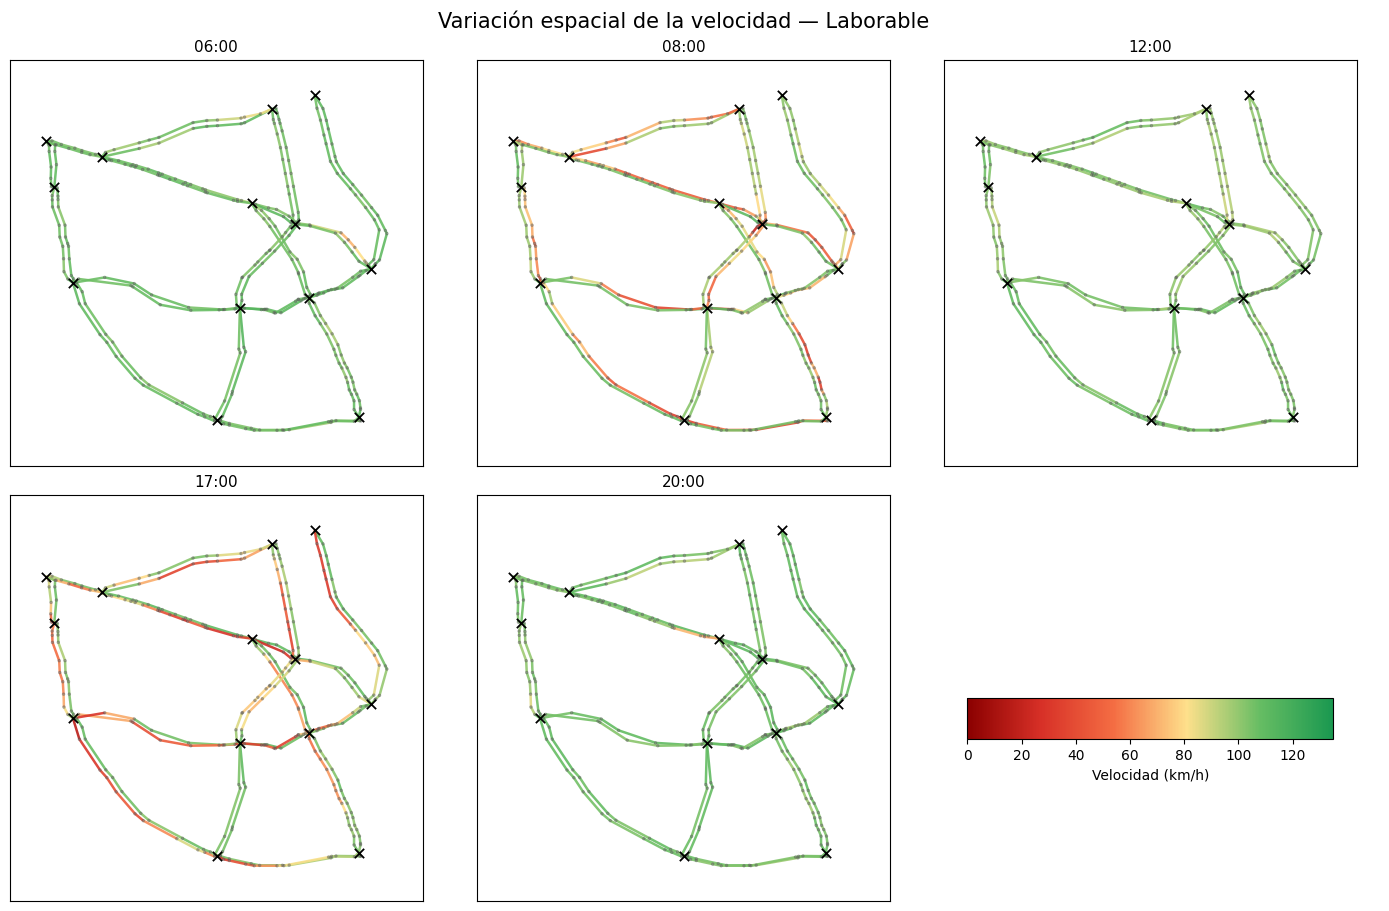
\includegraphics[width=0.92\textwidth]{figuras/variacion_espacial_dias_laborables.png}
    \caption{Variación espacial de la velocidad en la red experimental durante días laborables para cinco horarios representativos. Cada panel muestra la velocidad mediana de las aristas a la hora correspondiente y todos utilizan una misma escala de velocidad.}
    \label{fig:variacion_espacial_laborables}
\end{figure}

La comparación de estos estados muestra que las reducciones más pronunciadas de velocidad durante los días laborables se concentran alrededor de las 08:00 y las 17:00 horas, pero no afectan de manera uniforme a toda la red. A las 06:00, 12:00 y 20:00 predominan velocidades relativamente elevadas, mientras que durante las dos horas pico aparecen reducciones localizadas en diferentes corredores. Además, los dos sentidos de una misma autopista pueden presentar condiciones sustancialmente distintas en un mismo periodo, lo que indica que una representación agregada por autopista podría ocultar parte de la variabilidad presente en los datos.

El mismo procedimiento se aplicó a los fines de semana. En este caso, los cinco estados representativos mostraron una estructura espacial considerablemente más estable. Aunque se observaron algunas reducciones localizadas de velocidad, no apareció una reorganización espacial tan marcada como la registrada durante los días laborables. Esta diferencia es consistente con el perfil horario analizado en la sección anterior y refuerza la conveniencia de considerar conjuntamente la hora del día, el tipo de día y la ubicación dentro de la red. Por razones de espacio, se presenta en el cuerpo del documento únicamente la secuencia correspondiente a los días laborables; la visualización equivalente para fines de semana se conserva en el cuaderno computacional asociado con este avance.

Además de la inspección espacial, se realizó una comparación cuantitativa entre los corredores dirigidos durante las horas pico de los días laborables. Debido a que los distintos corredores presentan niveles habituales de velocidad diferentes, se definió para cada corredor $c$ una velocidad de referencia $v^{\mathrm{ref}}_c$, correspondiente al mayor valor mediano observado entre las 06:00, 12:00 y 20:00 horas. La reducción relativa observada durante una hora pico $h$ se calculó como

\[
r_c(h)
=
100
\frac{v^{\mathrm{ref}}_c-v_c(h)}
     {v^{\mathrm{ref}}_c},
\]

donde $v_c(h)$ representa la velocidad mediana del corredor $c$ en el horario analizado. Esta normalización permite comparar las reducciones relativas entre corredores aun cuando sus niveles habituales de velocidad sean diferentes.

La Tabla~\ref{tab:patron_direccional} resume, para cada una de las ocho autopistas representadas, el sentido que presenta la mayor reducción relativa a las 08:00 y a las 17:00. La comparación permite observar de manera directa si el sentido relativamente más afectado se mantiene o cambia entre las dos horas pico.

\begin{table}[htbp]
\centering
\small
\caption{Sentido con mayor reducción relativa de velocidad por autopista durante las horas pico de días laborables.}
\label{tab:patron_direccional}
\begin{tabular}{lccccc}
\hline
\textbf{Autopista} &
\textbf{Sentido 08:00} &
\textbf{Caída (\%)} &
\textbf{Sentido 17:00} &
\textbf{Caída (\%)} &
\textbf{Cambio} \\
\hline
17  & 17-N  & 13.2 & 17-N  & 4.7  & No \\
85  & 85-N  & 42.6 & 85-S  & 44.9 & Sí \\
87  & 87-N  & 30.1 & 87-S  & 36.4 & Sí \\
101 & 101-N & 47.4 & 101-S & 39.1 & Sí \\
237 & 237-W & 36.9 & 237-E & 46.5 & Sí \\
280 & 280-N & 31.4 & 280-S & 53.9 & Sí \\
680 & 680-N & 12.5 & 680-S & 47.7 & Sí \\
880 & 880-N & 21.6 & 880-S & 26.3 & Sí \\
\hline
\end{tabular}
\end{table}

Los resultados muestran un patrón direccional marcado. En siete de las ocho autopistas, el sentido con la mayor reducción relativa de velocidad a las 08:00 difiere del más afectado a las 17:00. En las autopistas con orientación norte--sur, la mayor reducción matutina se concentra predominantemente en el sentido norte, mientras que durante la tarde se desplaza hacia el sentido sur. En la autopista 237 se observa un comportamiento análogo entre los sentidos oeste y este. La autopista 17 constituye la principal excepción, ya que el sentido norte permanece como el relativamente más afectado en ambos horarios.

La autopista 101 permite apreciar con mayor detalle la magnitud de estas diferencias. A las 08:00, el corredor 101-N presenta una reducción de 47.4\,\% respecto de su velocidad de referencia, mientras que 101-S registra únicamente 1.9\,\%. A las 17:00 el patrón se invierte: la reducción alcanza 39.1\,\% en 101-S y sólo 0.7\,\% en 101-N. Por tanto, la diferencia no se limita a identificar cuál de los dos sentidos resulta relativamente más afectado, sino que muestra que ambos pueden experimentar condiciones sustancialmente distintas en un mismo horario.

En conjunto, la evidencia temporal y espacial muestra que las condiciones observadas de movilidad presentan variaciones asociadas con la hora, el tipo de día, la localización y el sentido de circulación. Por esta razón, los 156 pares origen--destino dirigidos se mantienen como variables diferenciadas en los experimentos posteriores. Esta heterogeneidad resulta también relevante para el escenario $K>0$, ya que distintas observaciones actuales pueden reflejar condiciones diferentes de la red y, por tanto, no necesariamente aportar la misma información para la reconstrucción de la matriz objetivo.

\section{Protocolo experimental y criterios de evaluación}

\subsection{División temporal de los datos}

La evaluación del baseline debe preservar el orden temporal de las observaciones. Debido a que el objetivo es estimar condiciones futuras a partir de información histórica previamente disponible, una partición aleatoria de los datos permitiría que observaciones correspondientes a fechas posteriores participaran en la construcción de referencias utilizadas para estimar fechas anteriores. Esto introduciría fuga de información y produciría una evaluación que no representaría adecuadamente el uso esperado del método.

Por esta razón, las 52\,116 observaciones temporales se dividieron cronológicamente en tres subconjuntos consecutivos: entrenamiento, validación y prueba. La partición se realizó sobre la representación tabular de los 156 pares origen--destino descrita en la Sección~2.3, por lo que cada instante y sus 156 tiempos asociados permanecen siempre dentro del mismo subconjunto.

La distribución resultante se presenta en la Tabla~\ref{tab:division_temporal}.

\begin{table}[htbp]
\centering
\small
\caption{División temporal utilizada en el protocolo experimental.}
\label{tab:division_temporal}
\begin{tabular}{llrr}
\hline
\textbf{Conjunto} &
\textbf{Periodo} &
\textbf{Observaciones} &
\textbf{Porcentaje} \\
\hline
Entrenamiento & Ene.--abr. 2017 & 34\,548 & 66.29\,\% \\
Validación    & Mayo 2017       & 8\,928  & 17.13\,\% \\
Prueba        & Junio 2017      & 8\,640  & 16.58\,\% \\
\hline
\textbf{Total} & Ene.--jun. 2017 & \textbf{52\,116} & \textbf{100\,\%} \\
\hline
\end{tabular}
\end{table}

El conjunto de entrenamiento comprende las observaciones desde el 1 de enero hasta el 30 de abril de 2017 y se utiliza para construir las referencias históricas consideradas durante el desarrollo del baseline. El conjunto de validación corresponde al mes de mayo y se utiliza para comparar alternativas de especificación y seleccionar la configuración de $K=0$. Finalmente, las observaciones de junio conforman el conjunto de prueba y se mantienen fuera de este proceso de selección hasta la evaluación final.

Esta separación permite distinguir dos decisiones experimentales. En primer lugar, la información del conjunto de validación puede utilizarse para decidir, por ejemplo, qué variables temporales, granularidad o estadístico histórico producen una mejor referencia. En segundo lugar, el desempeño final debe estimarse sobre un periodo posterior que no haya participado en esas decisiones. De esta manera, la comparación sobre el conjunto de prueba proporciona una evaluación fuera de muestra de la especificación seleccionada.

La partición conserva además el orden cronológico completo,

\[
\max(t_{\mathrm{entrenamiento}})
<
\min(t_{\mathrm{validación}}),
\qquad
\max(t_{\mathrm{validación}})
<
\min(t_{\mathrm{prueba}}).
\]

de modo que la construcción y evaluación del baseline reproducen la dirección temporal que existiría en una aplicación operativa: aprender de observaciones pasadas para estimar condiciones posteriores.

\subsection{Métricas y criterio de desempeño}

El desempeño de las estimaciones se evalúa comparando cada tiempo origen--destino estimado con el valor correspondiente de la matriz de referencia $T^{\tau}_{\mathrm{ref}}(t)$. Las métricas se calculan de manera conjunta sobre todos los pares origen--destino y todos los instantes pertenecientes al subconjunto evaluado. Por tanto, cada combinación entre instante y par dirigido constituye una observación individual del error.

Sea $y_m$ el tiempo de desplazamiento de referencia para una de estas observaciones y $\widehat{y}_m$ su estimación, con $m=1,\ldots,M$. El error absoluto medio (\textit{Mean Absolute Error}, MAE) se define como

\[
\mathrm{MAE}
=
\frac{1}{M}
\sum_{m=1}^{M}
\left|
\widehat{y}_m-y_m
\right|.
\]

Dado que los tiempos de desplazamiento se encuentran expresados originalmente en minutos, el MAE se calcula en esta unidad y posteriormente se convierte también a segundos para facilitar su interpretación. Esta métrica se adopta como criterio principal de comparación, ya que expresa directamente la magnitud promedio de la desviación entre los tiempos estimados y los valores de referencia.

Como medida complementaria se utiliza la raíz del error cuadrático medio (\textit{Root Mean Squared Error}, RMSE),

\[
\mathrm{RMSE}
=
\sqrt{
\frac{1}{M}
\sum_{m=1}^{M}
\left(
\widehat{y}_m-y_m
\right)^2
}.
\]

A diferencia del MAE, el RMSE incrementa la influencia de las desviaciones de mayor magnitud debido al término cuadrático. Su utilización permite verificar si una especificación que presenta un buen error absoluto promedio genera, al mismo tiempo, errores particularmente grandes en una fracción de las observaciones.

También se calcula el error porcentual absoluto ponderado (\textit{Weighted Absolute Percentage Error}, WAPE),

\[
\mathrm{WAPE}
=
100
\frac{
\sum_{m=1}^{M}
\left|
\widehat{y}_m-y_m
\right|
}{
\sum_{m=1}^{M}
|y_m|
}.
\]

Esta métrica expresa el error absoluto acumulado en relación con la magnitud total de los tiempos observados y proporciona una medida relativa que facilita interpretar el tamaño del error independientemente de la unidad empleada.

Para la comparación detallada de las especificaciones candidatas se incorpora además el percentil 95 del error absoluto,

\[
P_{95}
=
Q_{0.95}
\left(
\left|
\widehat{y}_m-y_m
\right|
\right),
\]

donde $Q_{0.95}$ representa el percentil 95 de la distribución de errores absolutos. Este indicador permite caracterizar la parte superior de la distribución: un valor de $P_{95}=x$ implica que el 95\,\% de los errores absolutos no supera $x$. En los resultados se expresa en segundos.

La selección del baseline $K=0$ se realiza utilizando el MAE sobre el conjunto de validación como criterio principal. El RMSE, el WAPE y el percentil 95 se utilizan como métricas complementarias para identificar posibles diferencias que no resulten visibles únicamente a partir del promedio absoluto. En particular, cuando dos especificaciones presentan valores de MAE muy próximos, estas métricas permiten examinar si alguna de ellas produce desviaciones de mayor magnitud o un comportamiento menos estable.

Como referencia mínima de comparación se utiliza la estimación histórica más simple, construida para cada par origen--destino sin condicionamiento temporal. Las especificaciones posteriores deben demostrar sobre el conjunto de validación que la incorporación de estructura temporal aporta una reducción efectiva del error respecto de esta referencia. Entre las alternativas que satisfacen esta condición, la especificación con el menor MAE de validación se selecciona como baseline $K=0$. El conjunto de prueba no interviene en esta decisión y se utiliza únicamente después de que la especificación ha sido fijada.

En las etapas posteriores, la evaluación de los métodos correspondientes al escenario $K>0$ incorporará también el tiempo requerido para producir la reconstrucción una vez disponibles las observaciones actuales. Este tiempo se distinguirá de la latencia asociada con la obtención de dichas observaciones desde una fuente externa. En el presente avance, cuyo objetivo es establecer la referencia de precisión para $K=0$, este criterio no interviene en la selección del baseline.

\section{Construcción y selección del baseline $K=0$}

\subsection{Definición del escenario sin observaciones actuales}

El escenario $K=0$ representa el caso en el que, para un instante que se desea estimar, el método no dispone de observaciones actuales de tiempos de recorrido. En consecuencia, la estimación debe construirse exclusivamente a partir de información histórica disponible antes del periodo evaluado. Este escenario constituye la referencia más restrictiva del componente de estimación y permite establecer cuánto puede explicarse únicamente mediante regularidades históricas antes de incorporar información actual en el escenario posterior $K>0$.

En este contexto, $K$ representa el número de observaciones actuales disponibles para el método de estimación. En el presente avance se estudia únicamente el caso $K=0$; por tanto, durante la estimación de un instante $t$ no se proporciona ninguna observación actual y las 156 entradas objetivo de $T^\tau_{\mathrm{ref}}(t)$ permanecen ocultas. La naturaleza y localización de las observaciones que estarán disponibles en el escenario $K>0$ formarán parte del diseño experimental posterior.

Para cada par origen--destino dirigido $(i,j)$, el objetivo consiste en obtener una estimación

\[
\widehat{T}^{\tau,(0)}_{ij}(t)
\]

a partir únicamente de las observaciones históricas anteriores y de las características temporales del instante que pueden conocerse sin disponer de observaciones actuales, como la hora o el día de la semana. La colección de las 156 estimaciones produce la matriz

\[
\widehat{T}^{\tau,(0)}(t)
=
\left[
\widehat{T}^{\tau,(0)}_{ij}(t)
\right],
\]

que constituye la reconstrucción de la matriz de tiempos de desplazamiento bajo el escenario sin observaciones actuales.

La matriz completa $T^{\tau}_{\mathrm{ref}}(t)$ permanece oculta durante este proceso y se utiliza únicamente después de generar la estimación, con fines de evaluación. De esta manera se reproduce experimentalmente la situación en la que los tiempos actuales de todos los pares origen--destino no están disponibles, aunque el conjunto de datos permita conocerlos posteriormente para calcular el error.

Las estimaciones históricas se construyen de manera independiente para cada uno de los 156 pares dirigidos. Esto permite conservar las diferencias entre orígenes, destinos y sentidos de circulación identificadas en el análisis exploratorio, en lugar de utilizar una única referencia común para toda la red. La información histórica del conjunto de entrenamiento se resume mediante distintos niveles de condicionamiento temporal y cada alternativa genera, para un instante dado, una estimación completa de los 156 tiempos origen--destino.

Como primer nivel de análisis se consideran tres referencias de complejidad creciente: una estimación histórica de cada par sin condicionamiento temporal, una estimación condicionada por la hora del día y una estimación condicionada conjuntamente por el día de la semana y la hora. Estas alternativas permiten estudiar progresivamente cuánto valor aporta incorporar la estructura temporal observada en la Sección~3 antes de explorar una granularidad temporal más fina.

Todas estas referencias se construyen exclusivamente con el conjunto de entrenamiento definido en la Sección~4.1 y se comparan sobre el conjunto de validación. El conjunto de prueba permanece sin utilizar durante esta etapa. Una vez identificada la información temporal relevante, se analizarán diferentes resoluciones y estadísticos históricos para determinar la especificación definitiva del baseline $K=0$.

\subsection{Relevancia de la información temporal}

Antes de seleccionar una granularidad temporal específica para el baseline, se evaluó cuánto aporta incorporar información sobre la posición temporal de cada observación. Para ello se compararon tres referencias históricas de complejidad creciente, manteniendo en todos los casos la media como estadístico de estimación y conservando una referencia independiente para cada uno de los 156 pares origen--destino dirigidos.

La primera alternativa utiliza, para cada par $(i,j)$, una única media calculada con todas sus observaciones del conjunto de entrenamiento. Si $\mathcal{D}_{ij}^{\mathrm{ent}}$ representa el conjunto de tiempos históricos disponibles para dicho par, la estimación puede expresarse como

\[
\widehat{T}^{\tau,(0)}_{ij}(t)
=
\frac{1}{\left|D^{\mathrm{ent}}_{ij}\right|}
\sum_{y\in D^{\mathrm{ent}}_{ij}} y.
\]

Esta referencia no distingue entre horas ni días y constituye el nivel mínimo de comparación definido en la Sección~4.2.

La segunda alternativa incorpora la hora del día. En este caso, para estimar un instante $t$ se utilizan únicamente las observaciones históricas del mismo par origen--destino registradas durante la misma hora. De esta manera, cada par dispone de 24 valores históricos de referencia en lugar de uno solo.

La tercera alternativa incorpora conjuntamente el día de la semana y la hora del día. Cada estimación se obtiene entonces a partir de observaciones correspondientes al mismo par, al mismo día de la semana y a la misma hora que el instante evaluado. Esta representación produce hasta $7\times24=168$ referencias temporales para cada par origen--destino.

Las tres alternativas se construyeron exclusivamente con las observaciones de enero a abril y se evaluaron sobre el conjunto de validación correspondiente a mayo. Debido a que el estadístico utilizado es el mismo en los tres casos, la comparación permite aislar el efecto de incorporar progresivamente estructura temporal a la estimación.

La Tabla~\ref{tab:relevancia_temporal} presenta los resultados obtenidos.

\begin{table}[htbp]
\centering
\small
\caption{Desempeño de las referencias históricas iniciales sobre el conjunto de validación.}
\label{tab:relevancia_temporal}
\begin{tabular}{lrrrr}
\hline
\textbf{Referencia} &
\textbf{MAE (s)} &
\textbf{RMSE (s)} &
\textbf{WAPE (\%)} &
\textbf{Mejora MAE (\%)} \\
\hline
Media histórica              & 85.04 & 157.75 & 14.03 & 0.00 \\
Media por hora               & 46.12 & 107.41 & 7.61  & 45.76 \\
Día de semana + hora         & 26.93 & 68.21  & 4.44  & 68.34 \\
\hline
\end{tabular}
\end{table}

La incorporación de la hora del día reduce el MAE de 85.04 a 46.12 segundos, equivalente a una mejora de 45.76\,\% respecto de la media histórica no condicionada. Esta reducción muestra que mezclar en una única referencia observaciones correspondientes a distintos momentos del día elimina una parte importante de la estructura recurrente presente en los tiempos de desplazamiento.

Al incorporar además el día de la semana, el MAE disminuye a 26.93 segundos y el WAPE a 4.44\,\%. La reducción del MAE respecto de la referencia no condicionada alcanza 68.34\,\%. El RMSE también disminuye progresivamente, desde 157.75 segundos en la referencia más simple hasta 68.21 segundos al considerar conjuntamente día de la semana y hora, por lo que la mejora no se limita al error absoluto promedio, sino que también se observa en las desviaciones de mayor magnitud.

Estos resultados son consistentes con el análisis exploratorio de la Sección~3. El perfil horario mostró diferencias claras entre distintos momentos del día y entre días laborables y fines de semana, mientras que el análisis espacial evidenció que dichas variaciones no ocurren de manera uniforme en toda la red. La evaluación sobre validación muestra ahora que incorporar explícitamente esta estructura temporal permite mejorar de forma sustancial la estimación de los tiempos origen--destino.

La comparación no determina todavía la granularidad temporal más adecuada. La referencia condicionada por día de la semana y hora utiliza intervalos de 60 minutos, por lo que observaciones separadas dentro de una misma hora reciben todavía una estimación idéntica. Dado que PEMS-BAY dispone de observaciones con una resolución nominal de 5 minutos, el siguiente paso consiste en evaluar si una representación temporal más fina produce mejoras adicionales sin reducir excesivamente el soporte histórico disponible para cada combinación temporal.

\subsection{Granularidad temporal y selección de la especificación}

La comparación anterior mostró que condicionar las estimaciones por el día de la semana y la hora permite aprovechar una parte importante de la estructura temporal presente en los datos. Sin embargo, la agrupación por hora asigna la misma referencia histórica a todas las observaciones comprendidas dentro de un intervalo de 60 minutos. Dado que PEMS-BAY dispone de observaciones con una resolución nominal de 5 minutos, se evaluó si una representación temporal más fina permite mejorar adicionalmente la estimación.

Para ello se mantuvo el condicionamiento por día de la semana y se compararon cuatro resoluciones temporales: 60, 30, 15 y 5 minutos. En cada resolución, las observaciones del conjunto de entrenamiento se agrupan de acuerdo con el día de la semana y con el intervalo temporal al que pertenece cada instante. Para cada uno de los 156 pares origen--destino se calcula entonces un valor histórico independiente dentro de cada grupo temporal.

Además de modificar la resolución, se compararon dos estadísticos para resumir las observaciones históricas de cada grupo: la media y la mediana. De esta forma se obtuvieron ocho especificaciones candidatas, correspondientes a las combinaciones entre cuatro resoluciones temporales y dos estadísticos. Todas las alternativas se construyeron exclusivamente con el conjunto de entrenamiento y se evaluaron sobre el mismo conjunto de validación utilizado en la sección anterior.

La Tabla~\ref{tab:candidatos_k0} presenta los resultados de las ocho especificaciones. Las alternativas se encuentran ordenadas de acuerdo con el MAE, que constituye el criterio principal de selección definido en la Sección~4.2.

\begin{table}[htbp]
\centering
\small
\caption{Desempeño de las especificaciones candidatas para el baseline $K=0$ sobre el conjunto de validación.}
\label{tab:candidatos_k0}
\begin{tabular}{lrrrr}
\hline
\textbf{Especificación} &
\textbf{MAE (s)} &
\textbf{RMSE (s)} &
\textbf{WAPE (\%)} &
\textbf{$P_{95}$ (s)} \\
\hline
Mediana 5 min  & 24.06 & 63.73 & 3.97 & 126.69 \\
Media 5 min    & 24.13 & 62.66 & 3.98 & 123.84 \\
Mediana 15 min & 24.20 & 64.06 & 3.99 & 127.37 \\
Media 15 min   & 24.32 & 63.04 & 4.01 & 124.87 \\
Mediana 30 min & 24.85 & 65.43 & 4.10 & 130.63 \\
Media 30 min   & 24.98 & 64.26 & 4.12 & 128.59 \\
Mediana 60 min & 26.80 & 69.88 & 4.42 & 143.04 \\
Media 60 min   & 26.93 & 68.21 & 4.44 & 139.03 \\
\hline
\end{tabular}
\end{table}

La Figura~\ref{fig:mae_candidatos_k0} muestra la misma comparación utilizando únicamente el MAE, lo que permite apreciar visualmente el efecto de aumentar la granularidad temporal y la cercanía entre las mejores especificaciones.

\begin{figure}[H]
    \centering
    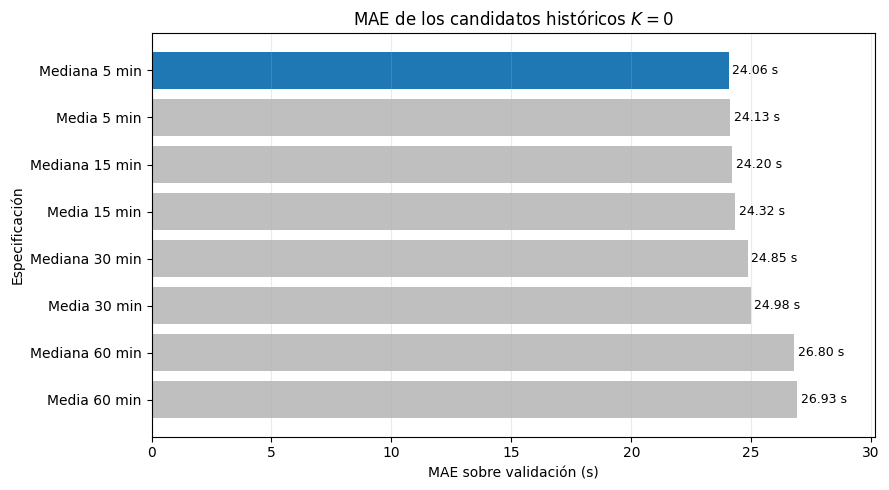
\includegraphics[width=0.88\textwidth]{figuras/mae_candidatos_k0.png}
    \caption{MAE sobre el conjunto de validación para las ocho especificaciones históricas candidatas del escenario $K=0$.}
    \label{fig:mae_candidatos_k0}
\end{figure}

Los resultados muestran una reducción progresiva del MAE conforme se utiliza una resolución temporal más fina. Las especificaciones de 60 minutos presentan errores cercanos a 27 segundos, mientras que las alternativas de 30 y 15 minutos reducen gradualmente este valor. Las dos especificaciones con resolución de 5 minutos presentan el menor MAE, lo que indica que la resolución temporal nominal de los datos conserva información útil que se pierde parcialmente al agregar observaciones en intervalos más amplios.

La diferencia entre los dos mejores candidatos es, sin embargo, muy pequeña. La mediana de 5 minutos obtiene el menor MAE, con 24.06 segundos, mientras que la media de 5 minutos alcanza 24.13 segundos, apenas 0.31\,\% por encima del mejor resultado. En contraste, la media de 5 minutos obtiene valores ligeramente menores de RMSE y del percentil 95 del error absoluto: 62.66 y 123.84 segundos, respectivamente, frente a 63.73 y 126.69 segundos para la mediana.

Esta diferencia es consistente con los estadísticos utilizados. La mediana minimiza el error absoluto dentro de cada grupo de observaciones y, por tanto, resulta particularmente apropiada cuando el MAE constituye el criterio principal de selección. La media, por su parte, se encuentra más directamente relacionada con la minimización del error cuadrático, lo que es consistente con el RMSE ligeramente menor observado para dicha alternativa. Debido a que el protocolo experimental estableció previamente el MAE como métrica principal, la pequeña ventaja de la mediana de 5 minutos determina la selección sin reinterpretar el criterio después de observar los resultados.

La utilización de resoluciones temporales más finas modifica tanto el número de grupos como la cantidad de observaciones individuales utilizadas para calcular cada referencia histórica. Con una resolución de 60 minutos se obtienen 168 combinaciones entre día de la semana e intervalo horario, con al menos 204 observaciones por grupo durante el periodo de entrenamiento. Sin embargo, cada una de estas combinaciones agrupa también las doce observaciones de 5 minutos contenidas dentro de una misma hora, por lo que ese número no representa 204 ocurrencias temporales independientes. Al utilizar resoluciones de 30 y 15 minutos se obtienen 336 y 672 grupos, con mínimos de 102 y 51 observaciones, respectivamente.

Con una resolución de 5 minutos se obtienen 2\,016 grupos temporales, cada uno respaldado por entre 17 y 18 observaciones históricas correspondientes al mismo día de la semana y a la misma posición temporal dentro del día. Esta granularidad elimina la agregación intrahoraria, pero conserva múltiples repeticiones históricas de cada contexto temporal. En el conjunto de validación no se observa un deterioro asociado con esta reducción del soporte por grupo; por el contrario, las especificaciones de 5 minutos presentan los menores valores de MAE. Por tanto, dentro del periodo analizado, la mayor resolución temporal permite conservar variaciones que se diluyen al utilizar intervalos más amplios sin producir una pérdida de desempeño en validación.

En consecuencia, se selecciona como baseline $K=0$ la mediana histórica de cada par origen--destino condicionada por el día de la semana y por el intervalo de 5 minutos correspondiente. Esta especificación obtiene un MAE de 24.06 segundos, un RMSE de 63.73 segundos, un WAPE de 3.97\,\% y un percentil 95 del error absoluto de 126.69 segundos sobre el conjunto de validación. En términos de MAE, representa una reducción de 71.71\,\% respecto de la media histórica no condicionada utilizada como nivel mínimo de referencia.

\section{Evaluación fuera de muestra}

\subsection{Resultados sobre el conjunto de prueba}

Una vez seleccionada la especificación del baseline $K=0$ mediante el conjunto de validación, se realizó una evaluación final sobre el periodo de prueba correspondiente a junio de 2017. En esta etapa ya no se comparan alternativas ni se modifica la configuración del método: se conserva la mediana histórica de cada par origen--destino condicionada por día de la semana e intervalo de 5 minutos, seleccionada en la Sección~5.3.

Antes de realizar la evaluación final, la referencia histórica se reestimó utilizando conjuntamente los datos de entrenamiento y validación, correspondientes al periodo de enero a mayo. Este procedimiento permite aprovechar toda la información histórica que estaría disponible antes del inicio del periodo de prueba sin incorporar ninguna observación de junio. La especificación del método permanece, por tanto, fija; únicamente se amplía el periodo histórico utilizado para calcular sus medianas de referencia.

El desempeño obtenido sobre junio se compara en la Tabla~\ref{tab:validacion_prueba} con el registrado previamente sobre el conjunto de validación.

\begin{table}[htbp]
\centering
\small
\caption{Desempeño del baseline $K=0$ en los conjuntos de validación y prueba.}
\label{tab:validacion_prueba}
\begin{tabular}{lrrrr}
\hline
\textbf{Periodo} &
\textbf{MAE (s)} &
\textbf{RMSE (s)} &
\textbf{WAPE (\%)} &
\textbf{$P_{95}$ (s)} \\
\hline
Validación (mayo) & 24.06 & 63.73 & 3.97 & 126.69 \\
Prueba (junio)    & 23.11 & 58.33 & 3.80 & 114.58 \\
\hline
\end{tabular}
\end{table}

Sobre el conjunto de prueba, el baseline obtiene un MAE de 23.11 segundos, un RMSE de 58.33 segundos, un WAPE de 3.80\,\% y un percentil 95 del error absoluto de 114.58 segundos. Estos valores son ligeramente inferiores a los obtenidos durante la validación, donde el MAE fue de 24.06 segundos y el RMSE de 63.73 segundos.

La ausencia de deterioro al pasar de mayo a junio indica que el desempeño observado durante la selección no depende exclusivamente del periodo de validación utilizado. En particular, el MAE permanece en un nivel similar y las métricas sensibles a errores de mayor magnitud, como el RMSE y el percentil 95, tampoco muestran un incremento en el conjunto de prueba. Este resultado proporciona evidencia de estabilidad fuera de muestra para la especificación seleccionada dentro del horizonte temporal analizado.

Al incorporar mayo al periodo histórico utilizado para construir la referencia final, cada combinación entre día de la semana e intervalo de 5 minutos dispone de entre 21 y 22 observaciones previas. Por tanto, la evaluación de junio continúa basándose exclusivamente en patrones históricos recurrentes y no utiliza ninguna observación actual de tiempos de recorrido.

El resultado de prueba establece así el nivel final de referencia del escenario $K=0$. Bajo las condiciones experimentales consideradas, una estimación de la matriz basada únicamente en información histórica alcanza un MAE de 23.11 segundos por entrada origen--destino. Este valor constituirá el punto de comparación para evaluar posteriormente si la incorporación de un número reducido de observaciones actuales, $K>0$, permite reconstruir con mayor precisión la matriz objetivo.

\subsection{Estabilidad y análisis del error}

La comparación entre validación y prueba permite examinar si la especificación seleccionada mantiene su desempeño al aplicarse a un periodo posterior que no intervino en su elección. Como se mostró en la Tabla~\ref{tab:validacion_prueba}, ninguna de las cuatro métricas evaluadas presenta deterioro al pasar de mayo a junio: el MAE disminuye de 24.06 a 23.11 segundos, el RMSE de 63.73 a 58.33 segundos, el WAPE de 3.97\,\% a 3.80\,\% y el percentil 95 del error absoluto de 126.69 a 114.58 segundos.

La comparación también permite examinar de manera preliminar la estabilidad de la especificación seleccionada al trasladarla a un periodo posterior. La resolución de 5 minutos fue elegida a partir de su desempeño sobre mayo y, posteriormente, la misma especificación se reestimó utilizando la información histórica disponible hasta el final de ese mes. Sobre junio no se observa deterioro en ninguna de las métricas evaluadas. Sin embargo, esta comparación debe interpretarse con cautela: se dispone únicamente de un mes de prueba y la referencia histórica utilizada para junio se construye con un mayor número de observaciones que la empleada durante la validación. Por tanto, los resultados aportan evidencia de estabilidad dentro del horizonte temporal analizado, pero no permiten descartar de manera concluyente posibles efectos de sobreajuste.

La relación entre las distintas métricas permite además caracterizar el error desde perspectivas complementarias. El MAE de 23.11 segundos representa la desviación absoluta promedio por entrada origen--destino, mientras que el RMSE de 58.33 segundos, al penalizar con mayor intensidad las desviaciones grandes, muestra que existen errores de magnitud superior al promedio. De forma consistente, el percentil 95 de 114.58 segundos indica que el 95\,\% de los errores absolutos se encuentra por debajo de aproximadamente 1.91 minutos. Por tanto, el desempeño promedio favorable no implica que todas las entradas de la matriz se estimen con una precisión cercana al MAE.

El WAPE de 3.80\,\% aporta una lectura adicional del error agregado respecto de la magnitud total de los tiempos de desplazamiento. Considerado junto con el MAE, el RMSE y el percentil 95, permite evitar que la evaluación del baseline dependa de una sola medida y muestra que la estabilidad observada entre validación y prueba se mantiene bajo criterios con distinta sensibilidad a la magnitud de los errores.

El análisis realizado en este avance es agregado sobre los instantes y los 156 pares origen--destino. En consecuencia, estas métricas permiten establecer el nivel global de desempeño del baseline, pero no identifican por sí mismas qué pares, horarios o condiciones de tráfico concentran las desviaciones de mayor magnitud. Realizar esa atribución requeriría un análisis adicional del error desagregado que no forma parte de la selección del baseline presentada en este avance.

En conjunto, los resultados no muestran deterioro fuera de muestra dentro del horizonte temporal analizado y proporcionan evidencia favorable sobre la estabilidad del baseline seleccionado. El baseline $K=0$ proporciona así una referencia histórica reproducible y suficientemente estable para la siguiente etapa del Proyecto, en la que se evaluará si la incorporación de un número reducido de observaciones actuales permite reducir el error de reconstrucción de la matriz.

\section{Conclusiones, alcance y transición al escenario $K>0$}

En este avance se construyó y evaluó un baseline para la estimación de la matriz de tiempos de desplazamiento en el escenario $K=0$, es decir, cuando el método de estimación no dispone de observaciones actuales de tiempos de recorrido. El objetivo no fue resolver todavía el problema completo de recuperación de rutas, sino establecer una referencia histórica reproducible que permita determinar cuánto de la matriz puede estimarse a partir de patrones temporales aprendidos previamente y contra la cual puedan compararse posteriormente métodos que incorporen información actual parcial.

Para ello se construyó un entorno experimental a partir de PEMS-BAY en el que las observaciones de velocidad se representan mediante una red dirigida y se transforman, mediante caminos de tiempo mínimo, en matrices de tiempos de desplazamiento entre 13 macronodos. Esta representación produce 156 pares origen--destino dirigidos para cada uno de los 52\,116 instantes disponibles entre enero y junio de 2017. El análisis exploratorio mostró que las condiciones de movilidad presentan estructura temporal, espacial y direccional, lo que justificó conservar estimaciones diferenciadas por par origen--destino y evaluar explícitamente distintas formas de condicionamiento temporal.

Los experimentos iniciales permitieron cuantificar la relevancia de dicha información temporal. Una media histórica no condicionada obtuvo un MAE de 85.04 segundos sobre el conjunto de validación. Al incorporar únicamente la hora del día, el error se redujo a 46.12 segundos, y al considerar conjuntamente el día de la semana y la hora disminuyó a 26.93 segundos. Posteriormente, la comparación de resoluciones de 60, 30, 15 y 5 minutos mostró que una representación temporal más fina proporciona mejoras adicionales.

De las ocho especificaciones evaluadas, la mediana histórica condicionada por día de la semana e intervalo de 5 minutos obtuvo el menor MAE de validación, con 24.06 segundos. Esta configuración se seleccionó utilizando exclusivamente el conjunto de validación y, una vez fijada, se reestimó con la información disponible de enero a mayo. Su evaluación final sobre junio produjo un MAE de 23.11 segundos, un RMSE de 58.33 segundos, un WAPE de 3.80\,\% y un percentil 95 del error absoluto de 114.58 segundos. La ausencia de deterioro respecto de validación aporta evidencia de estabilidad fuera de muestra dentro del horizonte temporal estudiado.

El baseline obtenido debe interpretarse dentro del alcance específico de este avance. Los tiempos utilizados como referencia experimental se derivan de la red construida a partir de PEMS-BAY y de los caminos de tiempo mínimo calculados bajo una representación instantánea del estado de la red. Por tanto, no constituyen mediciones directas de todos los tiempos origen--destino de una operación logística real. Asimismo, el análisis realizado evalúa globalmente los errores sobre los 156 pares dirigidos y no caracteriza todavía de manera sistemática qué pares, horarios o condiciones particulares concentran las desviaciones de mayor magnitud.

De igual forma, el baseline $K=0$ no constituye por sí mismo un mecanismo de detección de disrupciones ni un algoritmo de optimización o replaneación de rutas. Su función dentro de la arquitectura del Proyecto es proporcionar una estimación de los tiempos de desplazamiento que posteriormente puede ser utilizada como insumo por los mecanismos de monitoreo, evaluación de factibilidad y recuperación. En consecuencia, los resultados de este avance deben entenderse como el desarrollo y evaluación de uno de los componentes de información requeridos por el problema general de planeación y recuperación de rutas.

La siguiente etapa extiende esta formulación al escenario $K>0$. En dicho escenario, además del comportamiento histórico aprendido previamente, estarán disponibles únicamente $K$ observaciones actuales de tiempos de recorrido correspondientes a pares seleccionados de la red experimental. La naturaleza y localización de estas observaciones dependerán del método de reconstrucción y de la estrategia de selección que se adopten posteriormente. A partir de esta información se buscará actualizar la estimación histórica

\[
\widehat{T}^{\tau,(0)}(t)
\]

para obtener una reconstrucción más precisa de los tiempos origen--destino requeridos,

\[
\widehat{T}^{\tau,(K)}(t), \qquad K>0,
\]

sin requerir la observación directa de la totalidad de los 156 pares que conforman la matriz objetivo.

El problema experimental posterior tendrá, por tanto, dos dimensiones relacionadas: determinar cuánto mejora la reconstrucción al incrementar $K$ y estudiar qué observaciones actuales resulta más conveniente incorporar. La heterogeneidad temporal, espacial y direccional identificada en este avance sugiere que distintas observaciones pueden aportar cantidades diferentes de información, por lo que su selección constituye una parte relevante del problema y no únicamente su número.

El baseline desarrollado proporciona el punto de partida para esta comparación. Los métodos posteriores deberán evaluarse no sólo por su capacidad para reducir el error respecto del escenario puramente histórico, sino también considerando el número de observaciones actuales requeridas y el tiempo necesario para producir la matriz actualizada. Si un conjunto reducido de observaciones permite mejorar de manera suficiente la reconstrucción, la matriz resultante podrá incorporarse posteriormente al mecanismo de monitoreo y recuperación de rutas, manteniendo separado el componente de estimación de movilidad del modelo de optimización encargado de tomar las decisiones de replaneación.

\printbibliography
\end{document}